\chapter{Defining Mapbox Vector Tiles}\label{chapter_defining_mapbox_vector_tiles}

The main requirement regarding the content of the vector tiles is to be compatible with the vector tiles of Mapbox. This allows people to seamlessly switch to \osmvt{} and use the same visual styles created with Mapbox Studio. 

\section{Approach}
Mapbox's tileset is called Mapbox Streets. Mapbox provides detailed documentation on what data is included in the Mapbox Streets vector tiles. The documentation contains a layer reference which defines the attributes a layer can have. However the zoom levels at which data is shown is not documented publicly as well as the \osm{} tags and constraints describing the data. To be able to reverse engineer Mapbox Streets this information had to be retrieved by analyzing the official Mapbox Streets vector tiles at different zoom levels.\\
In an iterative and time consuming process the mapping and queries were continuously improved until the vector tile output matches the data from Mapbox Streets very closely.

\section{Implementation}
This section describes the main components which needed to be implemented in order to generate Mapbox Streets compatible vector tiles.

\begin{figure}[H]
\centering
\includegraphics[width=1.0\textwidth]{images/osm_to_vectortiles_detailed}
\caption{Simplified process from data import to vector tile rendering}
\end{figure}

\clearpage

\subsection{Import Mapping}

Imposm3\cite{4_github_2015} is used to import the \osm{} data into the PostgreSQL database. Imposm3 expects a definition of which \osm{} tags should be mapped to which database tables. This import mapping definition satisfies the two purposes of filtering and mapping the data.

\paragraph{Filter data} The mapping allows to filter explicitly by tags and defines which data is imported. This is important since only a subset of all \osm{} data is included in the vector tiles and  therefore not all \osm{} data needs to be imported.

\paragraph{Mapping data} The mapping allows to map \osm{} key/value pairs to a certain database table creating a structured and organized schema from semi-structured data. It takes care of constructing actual geometries from the \osm{} data model (\autoref{openstreetmap_data_model}).

\vskip 0.2in

The example definition in listing \autoref{definition_of_mapping} maps \osm{} tags with the key aeroway and one of the values runway, taxiway, apron or helipad to the table \textbf{aero\_polygon}. The \textbf{aero\_polygon} table has the columns id, geometry, timestamp and type. During the import process Imposm3 transformes the \osm{} nodes, ways and relations to one of the geometry types point, linestring or polygon. The mapping is one of the most important aspects of the project and maps more than 400 individual tags.

\begin{listing}[H]
\begin{yamlcode}
aero_polygon:
  type: polygon
  fields:
  - name: id
    type: id
  - name: geometry
    type: geometry
  - name: timestamp
    type: pbf_timestamp
  - name: type
    type: mapping_value
  mapping:
    aeroway:
    - runway
    - taxiway
    - apron
    - helipad
\end{yamlcode}
\caption{YAML definition of a single table in the import mapping}
\label{definition_of_mapping}
\end{listing}
\clearpage

\subsection{Zoom Level Views}\label{zoom_level_views}

After the import process all \osm{} data which is required for the vector tiles is stored in the database. Since only a subset of the data in the tables is shown on a given zoom level, SQL views for each zoom level and layer were created. The zoom level views filter the tables to the rows which are shown on a given zoom level.

\begin{figure}[H]
  \centering
  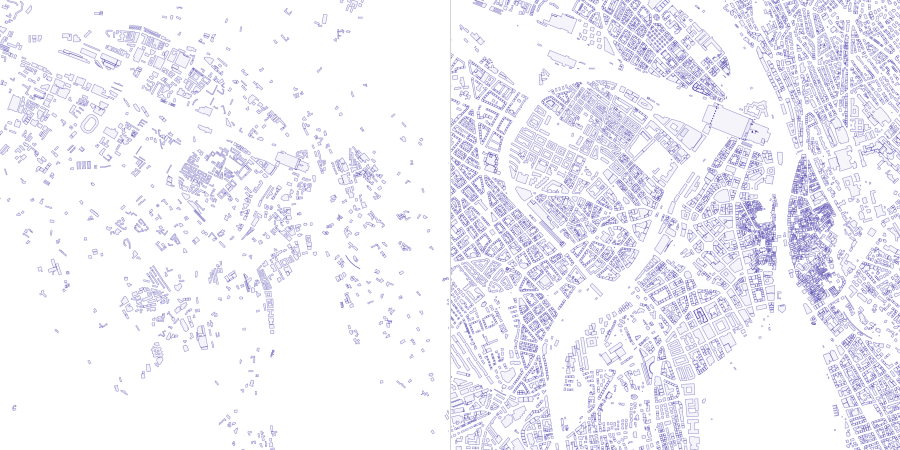
\includegraphics[width=\textwidth]{images/buildings_z13_z14}
  \caption{Difference of zoom level view 13 and 14 in buildings layer}
  \label{zoom_level_view_building_layer}
\end{figure}

\autoref{zoom_level_view_building_layer} shows on the left side the building layer on zoom level 13 and on the right side the same layer on zoom level 14. On zoom level 13 only a subset of the data, shown on zoom level 14, is visible. This example exactly shows the use of the zoom level views. 
\\
Listing \autoref{definition_of_zoom_level_view} shows the definition of the SQL views on both zoom levels. The \textbf{WHERE} clause in the query of the view \textbf{building\_z13} filters the rows to buildings which have an area greater than 1700. That is the reason why less buildings are shown in right side of \autoref{zoom_level_view_building_layer}.

\begin{listing}[H]
\begin{sqlcode}
CREATE OR REPLACE VIEW building_z13 AS
    SELECT id AS osm_id, underground, geometry
    FROM osm_building_polygon
    WHERE ST_Area(geometry) > 1700;

CREATE OR REPLACE VIEW building_z14 AS
    SELECT id AS osm_id, underground, geometry
    FROM osm_building_polygon;
\end{sqlcode}
\caption{Definition of zoom level views of building layer}
\label{definition_of_zoom_level_view}
\end{listing}

Additionally zoom level views help to decouple the database tables which hold the actual data and the definition of the layer. This is very helpful for example if new data is added to a layer, as only the import mapping and the zoom level view needs to be modified.

\subsection{Layer Definition}

The source project contains the definition of the layers inside the vector tiles. The definition contains metadata to access the database and a query which returns the necessary data for this layer. The listing \autoref{definition_of_layer} shows the definition of the layer \textbf{aeroway}. The query does not directly access the database table \textbf{aero\_polygon}. Instead it queries the zoom level views \textbf{aeroway\_z9} and \textbf{aeroway\_z10to14}.

\begin{listing}[H]
\begin{yamlcode}
- id: aeroway
    Datasource: 
      type: postgis
      table: |-
        (
          SELECT osm_ids2mbid(osm_id, is_polygon(geometry)) AS osm_id, geometry, type
          FROM (
            SELECT * FROM aeroway_z9
            WHERE z(!scale_denominator!) = 9
            UNION ALL
            SELECT * FROM aeroway_z10to14
            WHERE z(!scale_denominator!) BETWEEN 10 AND 14
          ) AS aeroway WHERE geometry && !bbox!
        ) AS data
    properties: 
      "buffer-size": 4
\end{yamlcode}
\caption{Definition of layer aeroway in the vector tile source project}
\label{definition_of_layer}
\end{listing}

This layer definition serves as input to the vector tile renderer (Mapnik). The tile renderer will execute every layer query for each tile and replaces expressions like \textbf{!scale\_denominator!} (zoom level) and \textbf{!bbox!} (extent of the tile) with the values of the current tile. If the query in listing \autoref{definition_of_layer} is executed for a tile on zoom level 8 it won't return any data as the \textbf{WHERE} clause will not match in both cases.
Whereas if it is executed on a tile on zoom level 9 all data of the zoom level view aeroway\_z9 will be included in the layer aeroway.

\begin{figure}[H]
\centering
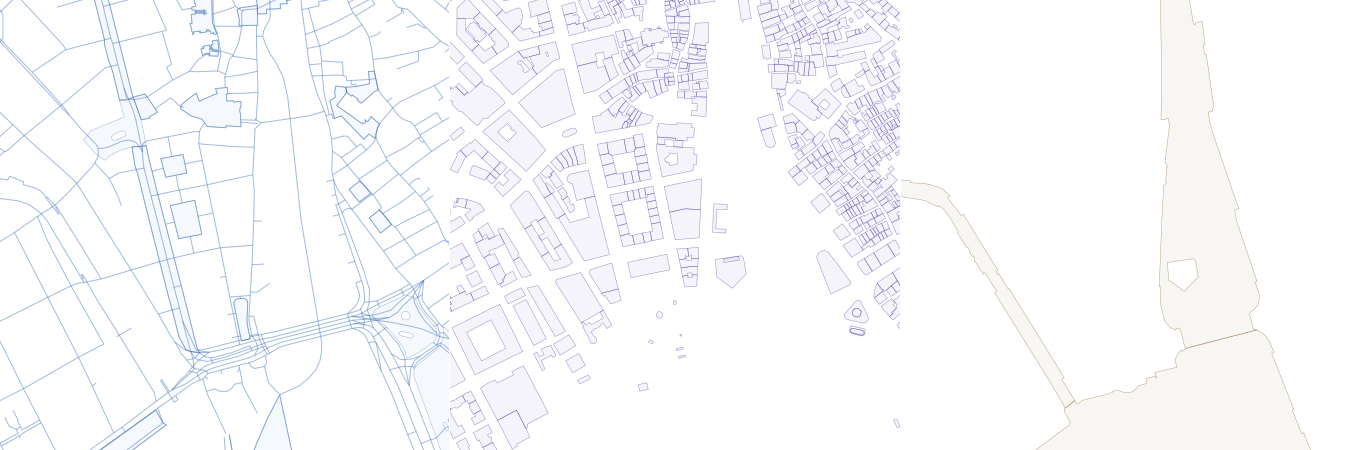
\includegraphics[width=\textwidth]{images/road_water_building}
\caption{Layer road, water, and building features on same map}
\end{figure}

\subsection{Relation between Database Tables, Zoom Level Views and Layers}

The \autoref{aero_db_schema} shows how the database tables, zoom level views and layers are related to each other. This architecture helps to structure the \osm{} data inside the database and opens the possibility to optimize single zoom levels individually. The arrow in \autoref{aero_db_schema} describes the data flow.

\begin{figure}[H]
\centering
\includegraphics[width=0.8\textwidth]{images/aero_database_schema}
\caption{Data flow between database tables, zoom level views and layer}
\label{aero_db_schema}
\end{figure}

\section{Problems and Optimizations}

During the development process of the map a number of problems were discovered and optimizations were implemented. This section explains the most interesting problems in detail.

\subsection{Avoid Expensive Transformations in Zoom Level Views}

The purpose of the zoom level views is to filter the data to only contain rows that are shown on a specific zoom level. Expensive calculations or transformations should be avoided in these views or made in a preprocessing step.\\

For example there are multiple label layers which transform a polygon geometry to a point geometry and since calculating the centroid from a polygon is expensive, transformations like these result in bad rendering performance.\\
The reason for this is that every time the layer query gets executed, all rows of the view get transformed even though only a subset of the data is needed for the rendered tile. Therefore selecting the right rows and only executing the transformation on this subset results in much better performance.



\begin{figure}[H]
\centering
\includegraphics[width=1.0\textwidth]{images/expensive_functions}
\caption{Move expensive function from zoom level view to layer definition}
\end{figure}


\subsection{Helper functions}

Small helper functions were created to make the queries more readable and secondly to reuse common logic through multiple queries.\\ 
Mapbox has introduced a complex classification schema to be able to filter features of a single layer. For example the layer landuse contains features of class park, school, cemetery and many more. This allows people to style these areas differently. OpenStreetMap has an entirely different data model. Therefore a helper function was created to assign the right class value to each row.

\begin{listing}[H]
\begin{sqlcode}
CREATE OR REPLACE FUNCTION landuse_class(type VARCHAR) RETURNS VARCHAR
AS $$
BEGIN
    RETURN CASE
        WHEN type IN ('park', 'dog_park', 'garden', 'playground') THEN 'park'
        WHEN type IN ('school', 'college', 'university') THEN 'school'
        WHEN type IN ('cemetery', 'christian', 'jewish') THEN 'cemetery'
    END;
END;
$$ LANGUAGE plpgsql IMMUTABLE;
\end{sqlcode}
\caption{Definition of classification helper function}
\label{definition_of_classification_helper_function}
\end{listing}

The listing \autoref{definition_of_classification_helper_function} shows the simplified class function of the layer landuse it takes the type value as input and returns the correct class value. 

\subsection{OpenStreetMap ID Transformation}

The data model of \osm{} consists of nodes, ways and relations. Every object gets its own OSM id assigned. This id is not unique across object types. Therefore one can find three objects with the same id but with a different object type.\\
While this works perfectly fine for \osm{}, this represents a problem because during the import process these \osm{} objects get transformed to PostGIS geometries. Objects of different types can get transformed to the same PostGIS geometry and therefore their ids would collide.
\\
In order to prevent this, the ids need to be transformed according to \autoref{osm_id_transformation} to make OSM ids unique within vector tiles \cite{103_mapbox.com_2016}.

\begin{table}[H]
\centering

\begin{tabular}{lll}
\hline
OSM type & Geometry type                  & \osm{} ID transform \\ \hline
node     & point                          & id x 10          \\
way      & linestring                           & (id x 10) + 1    \\
way      & polygon + polygon label points & (id x 10) + 2    \\
relation & linestring                           & (id x 10) + 3    \\
relation & polygon + polygon label points & (id x 10) + 4    \\
\end{tabular}
\caption{OSM id transformation}
\label{osm_id_transformation}
\end{table}

\subsection{Place Label Rank Calculation}\label{place_label_rank_calc}

Ranks are important for determining at which zoom level which places should be displayed. The NaturalEarth database contains places with scaleranks assigned by humans and is the most important source for better quality labels (historic places might be much more important despite having a very small population). This dataset is merged with the imported \osm{} data.
They can also be used to limit density at lower zoom levels to decrease data density.

\subsubsection*{Algorithm}

\noindent\begin{minipage}[t]{0.48\linewidth}
    \vspace{0pt}
    \begin{enumerate}  
        \item Divide map into grid
        \item Group labels by tile index
        \item Sort labels by scalerank, type and population within group
        \begin{enumerate}
            \item By scalerank ascending
            \item By type city, town, village, hamlet, suburb, neighbourhood
            \item By population descending
        \end{enumerate}
        \item Assign row number as \texttt{localrank}
    \end{enumerate}
\end{minipage}
\hfill
\begin{minipage}[t]{0.48\linewidth}
    \vspace{-10pt}
    \begin{figure}[H]
    \centering
    \includegraphics[width=\textwidth]{images/rank_calculation.png}
    \caption{Local place rank calculation}
    \end{figure}
\end{minipage}